\chapter{Transport calculations}
\label{app:transp}

Non-equilibrium Green's function (NEGF) calculations are now available with
{\dftbp}. Within this formalism it is possible to treat quantum mechanical
systems with open boundary conditions, i.e.\ systems connected to external
reservoirs and therefore quantum transport.  A new specific \kwcb{Transport}
block has been added to specify the geometry of such transport problems.
Additional solvers have been added to the \kw{Solver} section to either
fully solve the open boundary problem (using the keyword \kwcb{GreensFunction})
or the transmission through the system (\kw{TransportOnly}). Finally a
real-space Poisson solver is available for self consistent charge calculations
and electrostatic gates (within a new section, \kw{Electrostatics}, using the
keyword \kwcb{Poisson}).

\section{Definition of the geometry}
\label{sec:transport.geometry}

The input geometry for transport calculations can be a little tricky. In
comparison to cluster or supercell boundary conditions, the geometry for
transport calculation must also contain information about the contacts (external
reservoirs). The contacting leads (or surfaces) are actually semi-infinite
structures, supporting travelling waves. Unlike finite structures, where mo
stationary current is possible, travelling waves can only exist in such open
systems.  The simulation is therefore partitioned into a device region and two
or more contact regions.

Rules to build a valid input geometry:
\begin{enumerate}
\item \label{rule1} All device atoms must come first in the structure.
\item \label{rule2} Each contact must comprise of two subsequent unit cells,
  called principal layers (PLs). The two PLs together give all information about
  the contact structure and in the following are referred generally as a
  ``contact''.
\item \label{rule3} A PL is a unit cell of the contacting lead that has
  interactions only with its nearest neighbour PLs in tight-binding terms
  (i.e.\ the Slater-Koster interactions only extend into immediately neighbouring
  PLs).
\item \label{rule4} The ordering of the atoms within the two PLs of a contact
  must be consistent, in the sense that the two PLs must be exact periodic
  replicas of each other: If each PL comprise $N$ atoms, the $i^\mathrm{th}$
  atom in the first PL must have a corresponding identical atom, $i+N$, in the
  second PL which is related by translation to the position of atom $i$.
\item \label{rule5} The first PL in a contact should be always the one which is
  closer to the device region.
\item \label{rule6} All blocks should be contiguous in the structure and each
  atom must belong to one and only one region.
\item \label{rule7} The geometry can be defined as a cluster or a supercell. In
  the first case is it understood that the contacts are one-dimensional wire
  leads.
\item \label{rule8} If a structure is defined as being a {\em supercell}, only
  the lattice vectors that are transverse to the transport direction are
  meaningful. The periodicity specified along the transport direction is treated
  as a dummy vector (but must be present).
\item \label{rule9} For each contact the periodicity along the transport
  direction is actually deduced from the separation between the two PLs (using
  the coordinate difference $\mathbf{r}(i+N)-\mathbf{r}(i)$). We refer to this
  vector as aligned along the {\em contact direction}.
\item \label{rule10} All lattice vectors (including the contact direction
  vector) must be aligned parallel to one of the Cartesian axes $x$, $y$ or
  $z$. In practice only rectangular cells are allowed in transport calculations
  at present.
\end{enumerate}
An example of a non-periodic device with contacts attached is shown in
Figure~\ref{fig:device}.

\begin{figure}[!h]
  \begin{center}
    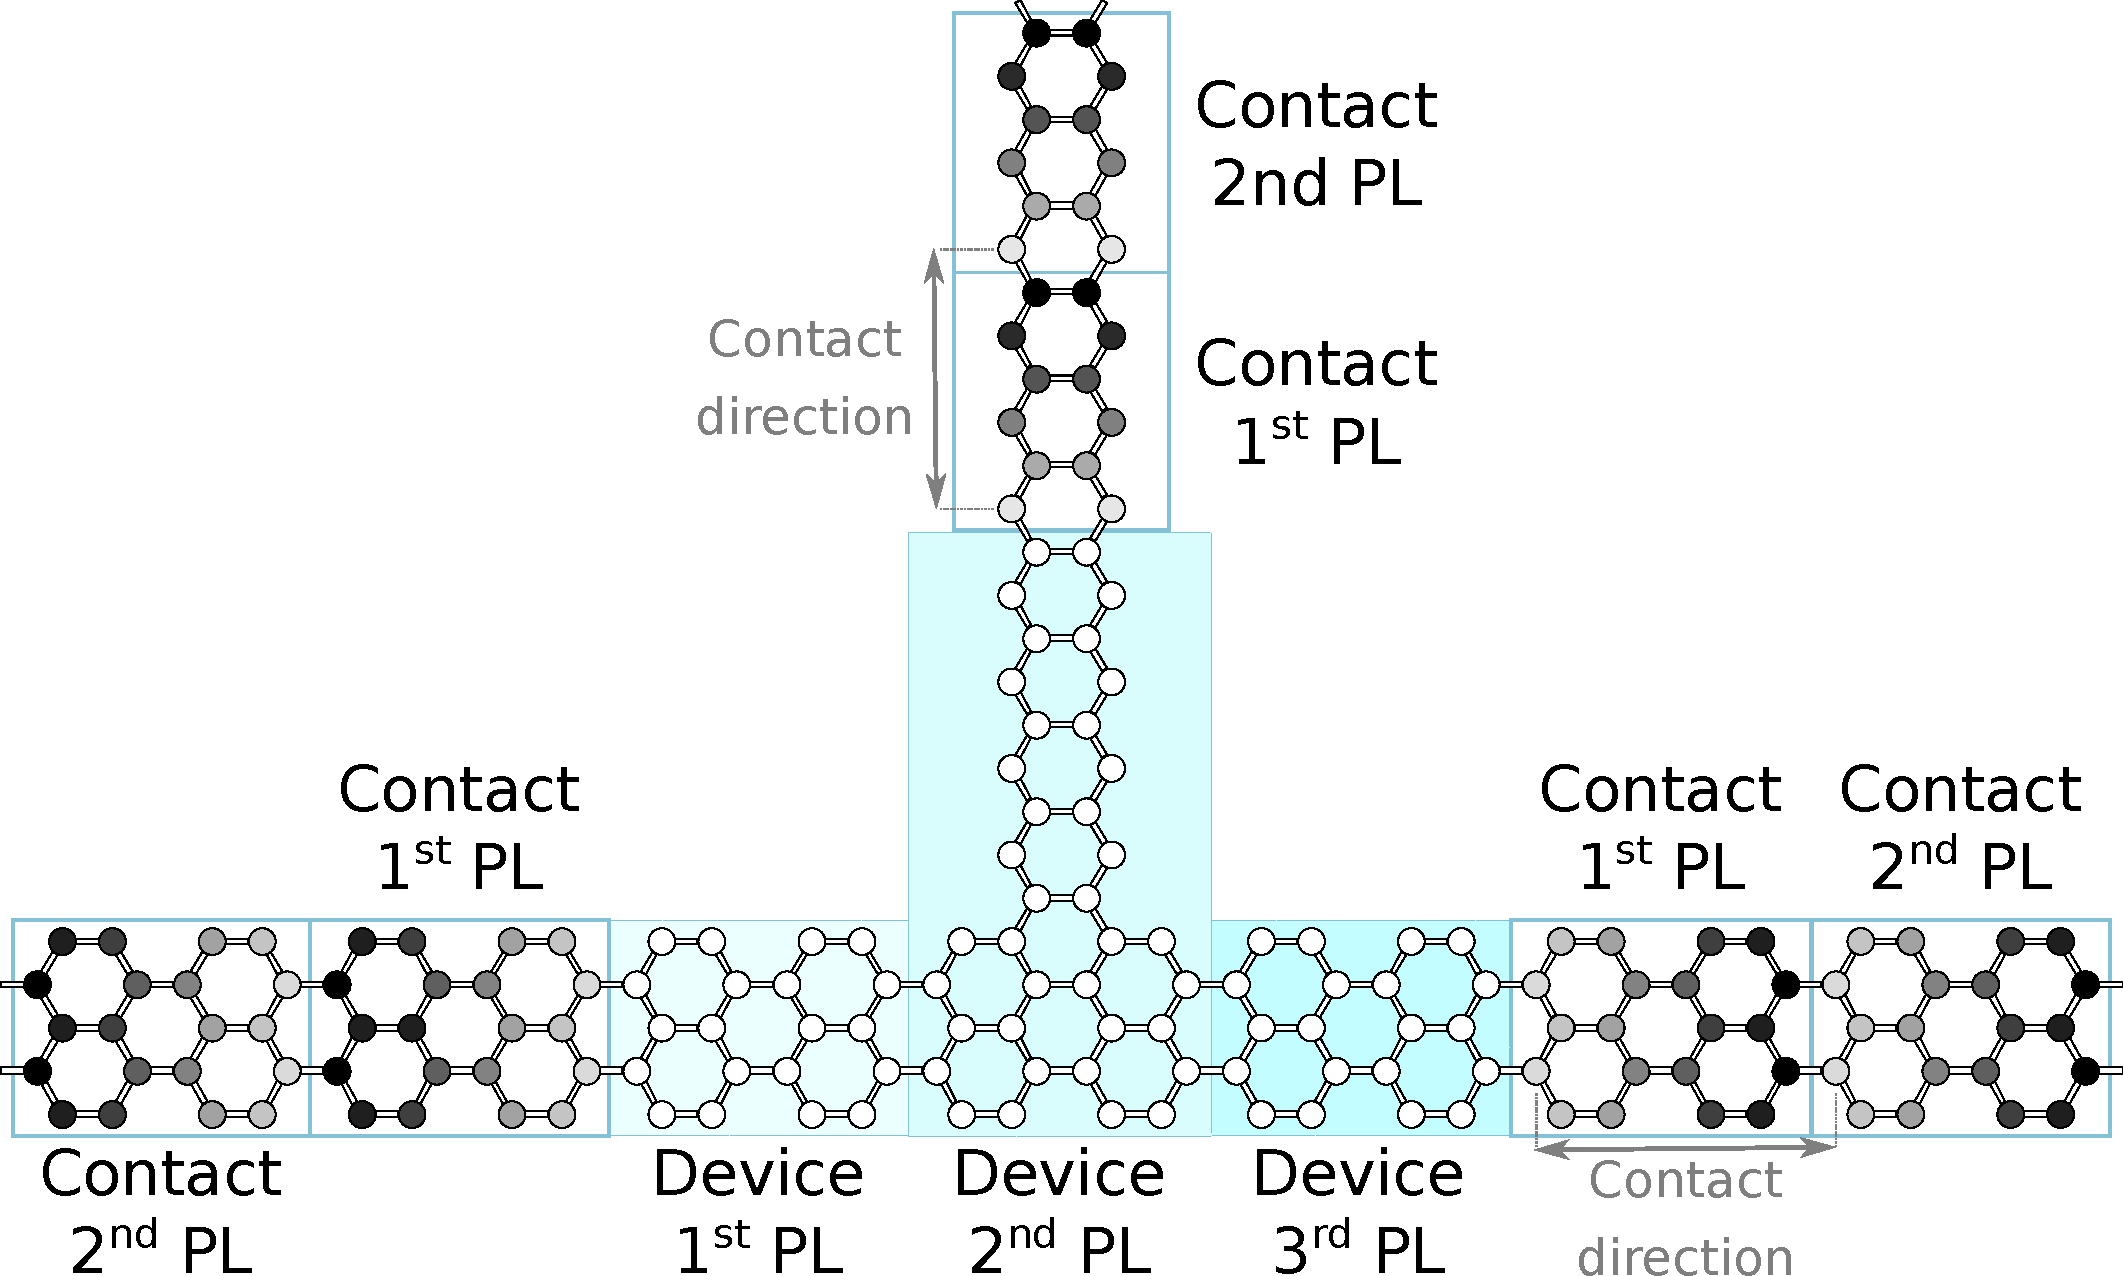
\includegraphics[width=0.8\textwidth]{Fig_device.pdf}
  \end{center}
  \caption{ \label{fig:device} Example of a valid 3 contact device with
    principal layers marked.}
\end{figure}

{\bf Note}:\\ The code {\em does not} currently check: if the device regions are
consistently defined (rules~\ref{rule1} and \ref{rule6}); if the PL defined are
really PLs (rule~\ref{rule3}); or if the first PL defined is really the one
closest to the device (rule~\ref{rule5}).\\ The code {\em does} check rules
\ref{rule4}, \ref{rule8}, \ref{rule9} and \ref{rule10}. The check for
rules~\ref{rule4} and \ref{rule9} is performed on the atomic coordinates, such
that
\begin{equation}
 \mathbf{R}^2_{i+N} = \mathbf{R}^1_i + \mathbf{v}\qquad\forall i \in PL
 \label{eqn:PLcriteria}
\end{equation}
where $\mathbf{R}^2_i$ are atomic coordinates of atoms in the second PL of the
contact, $\mathbf{R}^1_i$ are atomic coordinates of atoms in the first PL and
$\mathbf{v}$ is the contact lattice vector. The equality is verified within an
accuracy that can be set by the user (see below for \is{PLShiftTolerance}).

Please take care when building structures and to cross-check them. Also consider
looking at the examples distributed with the code. The input structure is often
the first suspect when there are problems in transport calculations.


\htsection{Transport}

The Transport section collects together the information needed whenever open
boundary conditions are used. It contains the description of the partitioning of
the system into a {\em device} and the {\em contact} regions and additional
information needed to calculate the required self-energies associated with the
contacts. The transport block contains the following properties:
\begin{ptable}
  \kw{Device} &p& & - & \pref{Device} \\
  \kw{Contact} &p& & - & \pref{Contact} \\
  \kw{Task} & m & & UploadContacts & \pref{Task} \\
\end{ptable}

An example transport geometry specification looks like:

\begin{verbatim}
Transport {
    Device {
      AtomRange = 1 8
    }
    Contact {
      Id = "source"
      AtomRange = 9 24
    }
    Contact {
      Id = "drain"
      AtomRange = 25 40
    }
}
\end{verbatim}

Where the associated atomic geometries follow the rules of
Section~\ref{sec:transport.geometry}. In this specific example, there is only
one principal layer in the device, but each contact contains two principle
layers (atoms 9--16 and 17--24 in the ``source'' contact, atoms 25--32 and
33--40 in the ``drain'' contact).

\htcbsubsection{Device}
The Device blocks contains the following properties:

\begin{ptable}
  \kw{AtomRange} &2i& & - & \pref{AtomRange} \\
  \kw{FirstLayerAtoms} &i+& & 1 &  \\
\end{ptable}

\begin{description}

\item[\is{AtomRange}] \label{AtomRange} defines the first and last atom of the
  device region.

\item[\is{FirstLayerAtoms}] defines the first atom of PLs in the device
  region. By default there is only one layer (the entire device
  region). Alternatively the user can manually reorder and group the atoms in
  the structure into distinct layers for more efficient Green's function
  calculations.

  The device layers, unlike the contact PLs, do not need to represent unit cell
  repetitions. If the device geometry has specified principal layers, these must
  be ordered in such a way that all the atoms within each of the layer are
  contiguous in space and adjacent layers must be placed next to each other in
  the structure. This ensures that the constructed hamiltonian and overlap are
  block tri-diagonal. Refer to~\cite{Pecchia_NJP} for a description of the
  efficient iterative Green's function algorithm that can then be applied.

\end{description}

\htcbsubsection{Contact} The contact block contains the following properties:

\begin{ptable}
  \kw{Id} & s &  & &  \\
  \kw{AtomRange} &2i& &  &  \\
  \kw{PLShiftTolerance} & r & & 1E-5 & \\
  \kw{Temperature} & r & & 0.0 & \\
  \kw{FermiLevel} &r& &  &  \\
  \kw{Potential} & r &  & 0.0 & \\
  \kw{WideBand} & l & & No & \\
  \kw{LevelSpacing} & r & WideBand = Yes & 0.735 & \\
  % these keywords are currently disabled:
  %\kw{WriteSelfEnergy} & l & & No & \\
  %\kw{ReadSelfEnergy} & l & & No & \\
  %\kw{ReadSurfaceGF} & l & & No & \\
  %\kw{WriteSurfaceGF} & l & & No & \\
\end{ptable}

The sections \verb|Device| and \verb|Contact| are used to define the atomic
range of each region. The user can also assign a label (\is{Id}) to each contact
that can be used later for cross referencing. In the section \verb|Contact| the
user can add a keyword that specifies the accuracy for the internal check of the
PLs (tolerance for rule~\ref{rule4} of structures, i.e.\ that accuracy to which
\eqref{eqn:PLcriteria} must be satisfied).

\begin{description}
\item[\is{Id}] Assign a text label to the contact (must be 50 or fewer
  characters).
\item[\is{AtomRange}]  Defines the first and last atom of the
  device region.  {\bf Note} the contacts should be defined such that the atoms
  included in the range are in continuous increasing order in the structure.
\item[\is{PLShiftTolerance}]\modif{\modtype{length}} Used to set the absolute
  accuracy used to check principal layer (PL) consistency (see above). The
  default is $10^{-5}$ atomic units. Please be aware that using a large values
  may hide errors due to an inconsistent definition of the contacts, therefore
  it should not be modified.
\item[\is{Temperature}]\modif{\modtype{energy}} Specifies the electronic
  temperature of the contact (see a more detailed discussion after the section 
  \"Analysis\").
\item[\is{FermiLevel}]\modif{\modtype{energy}} Optional over-riding of the Fermi
  energy specified in ther appropriate contact shift file.
\item[\is{Potential}]\modif{\modtype{energy}} Specifies any additional
  electrostatic potential applied to the contact. The natural units of this
  quantity are a potential energy.
\item[\is{WideBand}] Use the wide band approximation for the contact. If set to
  \is{Yes}, the surface Green's function of the contact is not explicitly
  calculated but is instead assumed to be local and constant according to a
  specified density of states.
\item[\is{LevelSpacing}]\modif{\modtype{energy}} Specifies the inverse of the
  density of states (DOS) per atom to be used for the Wide Band
  approximation. As an example, the DOS of gold at the Fermi level is
  0.05~eV$^{-1}$atom$^{-1}$, which corresponds to an energy spacing of 20~eV
  $\approx$0.735~Hartree (the default value).
%\item[\is{WriteSelfEnergy}] Write the contact's self energy to a binary file
%  matching its \is{contactId} and called \verb|contactId-SelfEnergy.mgf|.
%\item[\is{ReadSelfEnergy}] Read the contact's self energy from a binary file
%  matching its \is{contactId} and called \verb|contactId-SelfEnergy.mgf|.
%\item[\is{ReadSurfaceGF}] Read the contact's retarded Green's function from a
%  binary file matching its \is{contactId} and called
%  \verb|contactId-SurfaceGF.mgf|.
%\item[\is{WriteSurfaceGF}] Write the contact's retarded Green's function to a
%  binary file matching its \is{contactId} and called
%  \verb|contactId-SurfaceGF.mgf|.
\end{description}

\htcbsubsection{Task = ContactHamiltonian} \label{Task} The \is{Task} option is
used to define which type of calculation should be performed. Before performing
a transport calculation it is necessary to compute some equilibrium properties
of the contacts by running a periodic boundary condition DFTB calculation. This
necessary step must be carried out separately for each contact and can be done
by specifying a \kw{Task}=\is{ContactHamiltonian} block, as in the following
example to calculate the source case.

\begin{verbatim}
Task = ContactHamiltonian {
  ContactId = source
  ContactSeparation [Angstrom] = 50.0
}
\end{verbatim}

When \kw{Task}=\is{ContactHamiltonian} the following options can be defined

\begin{ptable}
  \kw{ContactId} & s &  & & \\
  \kw{ContactSeparation} & r & & 1e3 & \\
\end{ptable}

\begin{description}
\item[\is{ContactId}] Id label of the contact to be calculated.
\item[\is{ContactSeparation}]\modif{\modtype{length}} Dummy separation in
  transverse direction (see the following explanation).
\end{description}

The contact calculation computes the {\em bulk} Hamiltonian, self-consistent
charges (if SCC) and Fermi level for each contact. This is a usual \dftbp
calculation for which appropriate parameters must be included in the input
file. For {\em supercell} structures the calculation of the contact is performed
using corresponding supercells in which the transverse lattice vectors are those
specified in the \is{Geometry} tag and the lattice vector along the {\em contact
  direction} is deduced from the PL separations (rule~\ref{rule9}). If the
structure is defined as a {\em cluster}, the contact calculation is performed
for a {\em supercell} in which the contact is treated as one-dimensional
periodic wire with a surrounding vacuum region. However, since \dftbp does not
support pure one- and two-dimensional calculations, dummy lattice vectors are
defined for the two remaining directions. The default value for these lattice
vectors is 1000~a.u.\ (527~{\AA}), which should guarantee sufficient wire to
wire distances to avoid Coulomb interactions. The user can specify an
alternative contact separation using the keyword \is{ContactSeparation} placed
in the \kw{ContactHamiltonian} block.  Each contact computation produces one
output file called \verb|shiftcont_ContactId.dat| which storing energy shifts
and Mulliken charges that must be present in the working folder in all
subsequent transport calculations.

{\bf Note} that during the contact calculation you will need to perform a
k-point integration in the contact direction (as the contacts are
semi-infinite).  Whenever the system is defined as a cluster, \dftbp{} will
automatically extract the periodicity vectors from the geometry such that the
first reciprocal vector will correspond to the contact direction.  Therefore you
must specify a k-point sampling for the periodic calculation by sampling along
the first reciprocal lattice vector.  As an example, if the structure is defined
as a cluster (i.e., 1-dimensional wire leads), the source contact calculation
will have an input file similar to:

\begin{verbatim}
...
Task = ContactHamiltonian {
  ContactId = source
}
...
Hamiltonian = DFTB {
...
KpointsAndWeights = SupercellFolding {
     8  0  0   # sampling points here regardless of the transport direction
     0  1  0
     0  0  1
     0.5 0.0 0.0
  }
}
\end{verbatim}

On the other hand, if your structure is defined as a supercell (as an example, a
molecule with bulk contacts) and the transport direction is along the $y$
direction, your the source contact calculation will have an input file similar
to:

\begin{verbatim}
...
Task = ContactHamiltonian {
  ContactId = source
}
...
Hamiltonian = DFTB {
...
KpointsAndWeights = SupercellFolding {
     4  0  0   # points in periodic direction
     0  8  0   # points in transport direction
     0  0  4   # points in periodic direction
     0.5 0.5 0.5
  }
}
\end{verbatim}


This could seem confusing, but the underlining reasons is that in the cluster
calculation the reciprocal lattice is set up by the code itself, while in the
periodic calculation is set up by the user who can chose any arbitrary
direction.  Refer to the transport cookbook and to the distributed examples for
further clarification.

\htcbsubsection{Task = UploadContacts} After the contact calculations, it is
possible to perform actual transport calculations. This is activated simply
specifying \kw{Task = UploadContacts}, without additional options ({\bf Note} if
no task is specified, \dftbp{} assumes \is{UploadContacts} is the required task
in the transport block). In order to set up a proper transport calculation the
user should also define the contacts' Fermi levels (as printed in the files
previously produced by using \is{ContactHamiltonian} tasks) and any required
potential shift for each contact.
\begin{verbatim}
Transport {
  Device {
    AtomRange = 1 8
  }
  Contact {
    Id = "source"
    AtomRange = 9 24
    FermiLevel [eV] = -8.4123
    Potential = 0.0
  }
  Contact {
    Id = "drain"
    AtomRange = 25 40
    FermiLevel [eV] = -8.4123
    Potential = 1.0
  }
  Task = UploadContacts
}
\end{verbatim}

{\bf Note:} During the transport calculation you will not need to set up the
k-point integration when the structure is defined as a cluster, just as in a
regular \dftbp{} calculation. For supercell calculations, integration
perpendicular to the transport direction will need to be accurate, but the
sampling grid can in the transport direction itself can have only a single
value.  In the special case where your device is a supercell but also wire-like,
with a vacuum region lateral to its transport direction, the Gamma-point can be
chosen:
\begin{verbatim}
  KPointsAndWeights = {
    0 0 0  1.0
  }
\end{verbatim}

\htsection{GreensFunction}

For calculations in open systems, instead of calculating the eigenstates of the
system, a Green's function method is used to obtain the density matrix of the
system. The Green's function (GF) solver can also be used for conventional
supercell/cluster boundary conditions if required.

In order to activate Green's function calculations the user must define the
keyword \is{Solver = GreensFunction} in the \is{Hamiltonian} section. The
GF solver, either under equilibrium (no bias applied) or under non-equilibrium
conditions, builds the density-matrix of the device region such that it is
consistent with any contacts that are present. Strictly speaking the GF does not
solve for the eigenstates of the system, however it logically substitutes the
traditional construction of the density matrix from the eigenstates of the
system, as would be obtained after the diagonalisation step. The usual \dftbp{}
self-consistent calculations can be driven using the GF solver.

The following table gives the important parameters of the solver:
\begin{ptableh}
  \kw{Delta} & r  &  & 1E-5 & \\
  \kw{ContourPoints} & 2i &  & 20 20 &  \\
  \kw{LowestEnergy}  & r  &  & -2.0 & \\
  \kw{FermiCutoff}  & i & & 10 & \\
  \kw{EnclosedPoles} & i & & 3 & \\
  \kw{RealAxisStep} & r & RealAxisPoints=undefined & 6.65E-4 & \\
  \kw{RealAxisPoints} & r & RealAxisStep=undefined &  & \\
  \kw{SaveSurfaceGFs} & l & & Yes & \\
  \kw{ReadSurfaceGFs} & l & & No & \\
  \kw{FirstLayerAtoms} & i+ & Transport = undefined & 1 & \\
  \kw{FermiLevel} & r& Transport = undefined &  & \\
  \kw{LocalCurrents} & l&  & No & \\
\end{ptableh}

Note: For efficient GF calculation the device region must be partitioned into
layers whose fundamental property is to interact with nearest-neighbour layers
only (see section~\ref{sec:transport.geometry}).

\begin{description}
\item[\is{Delta}]\modif{\modtype{energy}} A small positive imaginary delta used
  in the GF definition and required for the x contour integration.
\item[\is{ContourPoints}] The number of points along the complex contour
  integration of the GF along the segments $\mathcal{C}$ and $\mathcal{L}$ (see
  contour integration in section~\ref{sec:transport.contourint}).
\item[\is{LowestEnergy}]\modif{\modtype{energy}} The initial energy from which
  the integration starts. It should be low enough to ensure that all the
  electronic states are correctly included in the integration. The default is
  -2.0 Hartree (see contour integration).
\item[\is{FermiCutoff}] Integer number setting the Fermi distribution cutoff in
  units of $kT$. It is read only if the Fermi distribution temperature is
  greater than 0 (see contour integration).
\item[\is{EnclosedPoles}] The number of Poles enclosed in the contour. It is
  meaningful only in finite temperature calculations (see contour integration).
\item[\is{RealAxisStep}]\modif{\modtype{energy}} The energy step along the real
  axis integration for non-equilibrium calculations. Note: \kw{RealAxisStep} and
  \kw{RealAxisPoints} cannot both be defined at the same time.

\item[\is{RealAxisPoints}] The number of points along the real axis integration
  needed in non-equilibrium calculations. The default depends on the electronic
  temperature and bias. Note: \kw{RealAxisStep} and \kw{RealAxisPoints} cannot
  both be defined at the same time.

\item[\is{SaveSurfaceGFs}] As the SCC cycle usually needs to repeat the
  calculation of the Green's function at given energy points and as the surface
  Green functions do not change during the SCC cycle, this flag allows for
  saving the surface Green functions to disk and so save computational time on
  every SCC cycle after the first.

\item[\is{ReadSurfaceGFs}] Loads the surface Green's function from a file at the
  the first SCC cycle. Note that this operation only makes sense if the energy
  integration points are identical to the calculation used to generate the
  surface Green's function files. The code does not verify whether this
  condition is fulfilled. In general there is no need to modify the defaults for
  \kw{ReadSurfaceGFs} and \kw{SaveSurfaceGFs}.

\item[\is{FirstLayerAtoms}] As described in Device block. Can be specified only
  if no \kw{Transport} block exists.  {\bf Note:} the Green solver can be used
  also to calculate the density matrix when there are no open boundary
  conditions, for example to take advantage of the iterative scheme in quasi-1d
  systems. In this case, a \kw{Transport} block is not defined and therefore
  \iscb{FirstlayerAtoms} should be given in the \is{GreensFunction} block. Also,
  the Fermi level of the system must be known and provided to fill up the
  electronic states.

\item[\is{FermiLevel}]\modif{\modtype{energy}} Required to set the Fermi level
  used by the Green's solver to fill up the electronic states, unless already
  specified by contacts being already present.

\item[\is{LocalCurrents}] if set to Yes, local bond-currents are computed using
  the non-equilibrium density matrix.  This task is currently limited to
  \textbf{non-periodic} systems. The output is placed in a file
  \verb|lcurrent_u.dat| (or \verb|lcurrent_d.dat| depending on spin).  The files
  are arranged in a table in order of increasing neighbour distance,

\begin{tabular}{|c|c|c|c|c|c|c|c|c|c|c|c|}
  \hline
  Atom(i) & x & y & z &  nNeighbours &  j1 & I$_{i,j1}$ & j2 & I$_{i,j2}$ &  j3 & I$_{i,j3}$ & ...\\
  \hline
\end{tabular}

  This file can be processed using the small code \verb|flux| provided in
  tools/transport that helps in building plots for jmol.
\end{description}

GreensFunction section example:

\begin{verbatim}
Solver = GreensFunction {
  FirstLayerAtoms = 1 61 92 145
  Delta [eV] = 1E-4
  ContourPoints = 20 20
  RealAxisPoints = 55
  LowestEnergy [eV] = -60.0
  FermiCutoff = 10
  EnclosedPoles = 3
}
\end{verbatim}


\section{Solver = TransportOnly}

The \is{GreensFunction} block is used to solve the full self-consistent NEGF
transport problem. However, the block \iscb{TunnelingAndDos} within the
\is{Analysis} block (see below), can be used to calculate the transmission
function according to the Landauer formula, without solving for the full density
matrix. This can be applied even for calculations where the density matrix and
charge densities are not computed. Similarly, in these cases the electrostatics
block should be omitted (i.e.\ the \is{Electrostatics = Poisson}). The keyword
\is{Solver = TransportOnly} is used to jump straight to the post-SCC
analysis.  \textbf{Note:} This option cannot be used together with calculations
which require forces, including geometry relaxations or md calculations.


\section{Contour integration}
\label{sec:transport.contourint}

Much of the computational work for transport is in the integration of the energy
resolved density matrix, as represented via the NEGF matrix. The integration is
efficiently performed with a complex contour integration and a real axis
integration, as shown in Figure~\ref{fig:contour} and discussed in
references~\cite{Pecchia_spring, Pecchia_RPP, Pecchia_NJP}.
\begin{figure}[!h]
  \begin{center}
    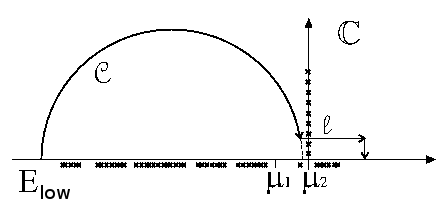
\includegraphics[width=8.0cm]{Fig_integration.png}
    \caption{ \label{fig:contour} Contour integration in the complex plane for
      the Green's functions. The crosses represent poles of either $G^r$ or the
      Fermi function.}
  \end{center}
\end{figure}
All integrations are performed with Gaussian quadratures and the number of
points must be specified manually. The complex contour integration is subdivided
into two sections: the first section is the arc of a circle, $\mathcal{C}$, that
can be computed with a few integration points (default 20); the second section
is a line that intersects the contour and runs parallel to the real axis at a
distance that depends on the number of poles of the Fermi function that are
enclosed within the contour. Usually a good choice for the number of poles is
between 3 and 5 (the default is 3). The poles are placed at the complex points
$z_m = E_F + i (2m+1) \pi k_B T$ and therefore are separated from each other by
$2 \pi k_B T$, where $k_B$ is Boltzmann's constant.  At $T=300$~K this
corresponds to a separation of 156~meV. It should be noted that, as the
temperature decreases, the separation between poles reduces. This makes the
contour integration harder as it needs to walk across two singularities. At very
low temperatures, $T=10$~K, the separation is 5.2~meV. Below this temperature,
the contour integration is treated as $T=0$ in order to avoid numerical
inaccuracies. The integration along the segment $\mathcal{L}$ extends up to
$Re\left[ z \right] = E_F + n k_B T$, where $n$ is an integer number specified
by the keyword \kw{FermiCutoff} and has a default value of 10.  In the limit
$T=0$~K the poles collapse into a non-analytic branch cut and the contour needs
to be changed such that the second section of the complex contour becomes the
arc of circle closing on the real axis.  Finally, the real axis integration
extends between the lowest and highest chemical potentials. The number of
quadrature points should depend on the bias itself and can be set using
\kw{RealAxisPoints} or \kw{RealAxisStep}. The default value is $1\text{~pt} /
0.018\text{~eV}$ (actually $1500\text{~pt} / 1\text{~Hartree}$). In finite
temperature calculations the segment is extended to include the Fermi cutoff by
$n k_B T$ on both sides ($\mu_1 - n k_B T, \mu_2 + n k_B T$). In this case the
number of quadrature points are increased by assuming the same point density
defined in the range ($\mu_1, \mu_2$).  Example: for a bias of 0.2~V, the
default number of points is $0.2 \cdot 1500 / 27.21139 = 11$. At $T=300$~K the
interval is increased by 0.26~eV on both sides, therefore $0.26 \cdot 1500 /
27.21139 = 14.33$ which is truncated to 14 points, leading to a total of 38
points along the real axis. The use of the keyword \kw{RealAxisStep} is usually
more convenient because it ensures a consistent real axis integrations during,
for example, a bias sweep.

Note: The GF solver can be used also for calculations other than the transport
context. In cases where the position of the Fermi Energy is known with good
accuracy, the density matrix solver based on the GF can be used to compute the
electronic properties of clusters and supercells. The recursive algorithm may be
an efficient solution to large problems having an elongated one dimensional
shape.

\section{Spin-polarised transport}

Spin-polarised transport is not available yet. Collinear spin transport will be
available soon, as all the needed machinery has been implemented and is
undergoing debugging and testing.


\section{Poisson solver}

The Poisson solver is a fundamental part of charge self-consistent
non-equilibrium transport calculations and must be declared whenever an SCC NEGF
calculation is performed using \is{Electrostatics = Poisson}. Under
non-equilibrium conditions the self-consistent potential of the KS equations
cannot be solved using the efficient $\gamma$-functional, but instead requires
the definition of appropriate boundary conditions for the potentials imposed by
the contacts. However, since the $\gamma$-functional is functionally related to
a pure Hartree potential, it can be obtained in real space by solving a Poisson
solver.  The Poisson equation is solved in a {\em box} with hexahedral prism
shape. This restriction is imposed by the Poisson solver being employed. This
restricts calculations of supercell structures to orthorhombic super-lattices.
An additional restriction is that the box sides must be aligned with the
Cartesian axes, $x$, $y$, $z$.

\begin{ptableh}
  \kw{Verbosity} & i & & 51 & \\
  \kw{PoissonBox} & 3r & &  &  \\
  \kw{BoxExtension} & r &  & 0.0 &  \\
  \kw{MinimalGrid} & 3r  &  & 0.5 0.5 0.5 & \\
  \kw{PoissonAccuracy} & r &  & 1E-7 &  \\
  \kw{AtomDensityTolerance}  & r  &  & 1E-6 & \\
  \kw{AtomDensityCutoff}  & r  &  & 14.0 & \\
  \kw{CutoffCheck} & l & & Yes & \\
  \kw{NumericalNorm}  & l  &  & No & \\
  \kw{SavePotential} & l & & No & \\
  \kw{PoissonAccuracy} & r & & 1E-6 & \\
  \kw{MaxPoissonIterations} & i & & 60 & \\
  \kw{BuildBulkPotential} & l & & Yes & \pref{Boundary Conditions}\\
  \kw{ReadOldBulkPotential} & l & & Yes & \pref{Boundary Conditions} \\
  \kw{OverrideDefaultBC} & m & & none\{\} & \pref{Boundary Conditions}\\
  \kw{OverrideBulkBC} & m & & none\{\} & \pref{Boundary Conditions}\\
  \kw{BoundaryRegion} & m & & global\{\} &  \pref{Boundary Conditions} \\
  \kw{Gate} & m & & none\{\} & \pref{Electrostatic Gates} \\
  \kw{MaxParallelNodes} & m & & none\{\} & \pref{Parallelisations} \\
  \kw{RecomputeAfterDensity} & l & & No & \\
  \kw{PoissonThickness} & r & contacts = 1 & &\\
\end{ptableh}


\begin{description}
\item[\is{Verbosity}] This parameter controls the level and amount of output
  messages and takes values ranging from 1 to 100.
\item[\is{PoissonBox}]\modif{\modtype{length}} Dimension of the Poisson box
  along the directions $x$, $y$ and $z$.
\item[\is{BoxExtension}]\modif{\modtype{length}} With this value it is possible
  to tune the position of the box interface between the device and contacts.  By
  default (\is{BoxExtension}=0.0) the boundary is placed at the midpoint between
  the last device atom and the first contact atom.
\item[\is{MinimalGrid}]\modif{\modtype{length}} The minimal requested grid
  spacing along $x$, $y$ and $z$. The actual grid spacing chosen by the
  multigrid solver will be lower than this.
\item[\is{AtomDensityTolerance}] In order to calculate the potential, the
  Mulliken charges are projected on the real space grid. This parameter defines
  the cutoff after which the charge is considered to vanish (i.e., the spatial
  extension of the projected charge). The default is 1E-6~e. Note that the
  contacts must be at least twice the length over which a projected Mulliken
  charge extends. If this conditions is not fulfilled and \is{CutoffCheck} is
  set to \is{Yes}, the code will exit with an error message. Setting this
  parameter to a lower value could allow shorter contacts to be defined in some
  cases. However this could lead to error in the potential and hence to spurious
  reflections, therefore it should be left at its default value (or changed very
  carefully).
\item[\is{AtomDensityCutoff}]\modif{\modtype{length}} Defines the atomic radius
  cutoff. This is an alternative to \is{AtomDensityTolerance} and directly
  specifies the distance over which charge density associated with an atom is
  considered to vanish.
\item[\is{CutoffCheck}] If set to \is{No}, consistency between contact length
  and charge extension is not verified (see \is{AtomDensityTolerance} and/or
  \is{AtomDensityCutoff}). The default is \is{Yes}. As with
  \is{AtomDensityTolerance}, this parameter should not be changed unless you
  know exactly what you're doing.
\item[\is{SavePotential}] Save the electrostatic potential to the file
  \verb|potential.dat| and the charge density to \verb|charge_density.dat|.
  Additional files \verb|Xvector.dat|, \verb|Yvector.dat|, \verb|Zvector.dat|
  and \verb|box.dat| are also created. These files can be converted to a cube
  file that can be visualised in jmol. See section~\ref{sec:transport.tools}
  about transport tools.
\item[\is{PoissonAccuracy}] Defines the accuracy for the approximate solution of
  the Poisson equation (default value 10$^{-6}$).
\item[\is{MaxPoissonIterations}] Defines the maximum number of iterations allowed
  for the solver.
\item[\is{RecomputeAfterDensity}] When set to \is{Yes}, Poisson's equation is
  solved again after the density matrix is created in order to make the
  electrostatic energy consistent with the newly updated charges.  In transport
  calculations it is set to \is{No} by default in order to avoid the extra time
  spent on the Poisson step. This does not affect the SCC loop or other
  calculations apart from the electronic energy and forces.
\item[\is{PoissonThickness}] In the special case of a single contact (cases like
  the end of semi-infinite wires or surfaces of crystals), the thickness of the
  Poisson box normal to the surface of the contact can be set with this command.
\end{description}

{\bf Note}: The Poisson box can be specified using the keyword
\verb|PoissonBox|. In calculations where two contacts face each other along the
same axis, setting the box-size along this axis will has no effect (the code
adjusts to the correct size internally). The \is{PoissonBox} keyword is
redundant (and should not be specified) when the system is periodic, since in
this case the box geometry is taken from the supercell lattice vectors.

Numerical error in the potential will results in spurious discontinuities at the
contact-device interfaces. The default tolerances should be sufficient to avoid
this in most cases.

Below is a a typical example of the whole Poisson block specification. Some of
the keywords are described in the next subsections.
\begin{verbatim}
 Electrostatics = Poisson {
  PoissonBox [Angstrom] = 20.0 20.0 20.0
  MinimalGrid [Angstrom] = 0.3 0.3 0.3
  SavePotential = No
  BuildBulkPotential = Yes
  ReadOldBulkPotential = No
  BoundaryRegion = Global {}
  PoissonAccuracy = 1E-7
  Gate = Planar{
      GateLength_l [Angstrom] = 10.0
      GateLength_t [Angstrom] = 20.0
      GateDistance [Angstrom] = 7.0
      GatePotential [eV] = 1.0
  }
}
\end{verbatim}

\htsubsection{Boundary Conditions}

The Poisson equation is solved imposing boundary conditions (BC) on the
potential at the six faces of the Poisson Box. In transport calculations for
non-supercell geometries comprising two contacts placed along the same axis, the
BCs are chosen as follows:
\begin{itemize}
\item[Dirichlet] fixed potentials on the two contact faces with values defined
  by the applied potentials (see \is{UploadContacts}).
\item[Neumann] zero normal field on the remaining 4 lateral box faces
\end{itemize}
In periodic supercells the BCs are: {\bf Dirichlet} (fixed potentials) on the
two contact faces with values defined by the applied potentials (see
\is{UploadContacts}) and {\bf Periodic} on the remaining 4 lateral box faces.

In some specific cases Neumann BCs can be set on one contact. In order to do so
it is necessary to use \is{OverrideDefaultBC} (see below).

The device and contact potentials should smoothly join at the interface. In
order to achieve this the code computes the bulk potential of each contact and
uses the result as a BC on the contact face of the Poisson box. This is useful
when the contact potential is not uniform due to charge rearrangements. Any
externally applied contact potential (\kw{Potential}) is added to the bulk
potential.  The user can deactivate this calculation by setting the keyword
\kw{BuildBulkPotential} to \is{No}.

{\bf Note}: The bulk potential is computed on a special box that has ``lateral''
sizes copied from the device box, and has the size of one PL along the contact
direction. The BCs are---so to speak---inherited from the device region. In
particular:
\begin{enumerate}
\item Along the contact direction periodic BCs are imposed on both faces.
\item On the other four faces the BCs are copied from the device region
  (supercell or cluster).
\item The user can override this setting using \verb|OverrideBulkBC| (see
  below).
\item When all four faces inherit Neumann BC (default for the device region),
  these are {\em ALL} internally changed to Dirichlet, because the solver cannot
  handle this situation as it gives rise to a singular matrix.
\end{enumerate}

\begin{description}
\item[\is{BuildBulkPotential}] (default: \is{Yes}) is used to calculate the
  electrostatic potential of the contacts and the result is used as a Dirichlet
  boundary condition on the contact face (superimposed to the contact
  potential).
\item[\is{ReadOldBulkPotential}] Read a previously computed bulk potential from
  hard-disk.
\item[\is{BoundaryRegion}] Specifies how the Dirichlet boundary conditions are
  treated on each contact face of the Poisson box. It can be \kw{Global},
  \kw{Square} or \kw{Circle}. \kw{Global} means that the BC is applied to the
  entire face of the box, whereas the other keywords imply that the Dirichlet BC
  are applied on a cross-section projected on the contact face. This is useful
  for instance when handling nanowire contacts, for which it is not really
  correct to impose a constant potential on the whole face of the Poisson box.
\item[\is{BufferLength}]\modif{\modtype{length}} can be used to set the size of
  the boundary region beyond the atomistic size which is determined as the
  minimal circle or square containing all atoms of the contact cross-section.
\end{description}

\begin{ptableh}
  \kw{BufferLength} & r &  & 9.0 &  \\
\end{ptableh}

Example:
\begin{verbatim}
BoundaryRegion = Circle {
    BufferLength [Angstrom] = 3.0
}
\end{verbatim}

In some special cases it might be necessary to override the default BCs applied
by the code to the Poisson equation. Currently this can be done using the
keywords: \verb|OverrideDefaultBC| and \verb|OverrideBulkBC|.

In the special case of a single contact, the boundary condition on the other
side of the box to that contact is automatically over-ridden to be of Neumann
type (but can still then be over-ridden with \is{OverrideDefaultBC}).

\begin{description}
\item[\is{OverrideDefaultBC}] block is used to override the BCs described
  above. It can be used to force Dirichlet or Neumann BCs along some specified
  directions or on one of the four lateral faces of the Poisson box.
\item[\is{Boundaries}] is used to specify on which face different BCs must be
  imposed. Assuming contacts are aligned along $z$, the keyword can be set to be
  any of \is{xmin}, \is{xmax}, \is{x}, \is{ymin}, \is{ymax} or \is{y}.
\end{description}

\begin{verbatim}
OverrideDefaultBC = Dirichlet {
      Boundaries = xmin
}
\end{verbatim}

For instance, setting a Dirichlet BC on \verb|Boundaries = xmin| imposes
$\phi(x,y,z)=0$ on the face placed at $x=x_{\text{min}}$, while
\verb|boundaries = xmax| would impose $\phi(x,y,z)=0$ on the face placed at
$x=x_{\text{max}}$. When Dirichlet needs to be forced on both faces it is
possible to use either \verb|boundaries = xmin,xmax| or simply
\verb|boundaries = x|. The same syntax can be used to impose conditions on more
faces, using \verb|boundaries = x,y| or \verb|boundaries = x,ymin|.

A similar strategy can be used to impose different boundary conditions on the
contacts. For instance, a Neumann BC can be set on one contact face by using

\begin{verbatim}
OverrideDefaultBC = Neumann {
      Boundaries = zmin
}
\end{verbatim}

{\bf Note} that the user should know which face of the Poisson Box corresponds
to the desired contact. Furthermore, if the user sets Neumann at all contacts
the Poisson solver will not converge (singular matrix) unless the Dirichlet
condition is imposed somewhere else (e.g., a gate potential is present).

It is also possible to override the default BCs when computing the bulk
potential.

\begin{description}
\item[\is{OverrideBulkBC}] block is used to override bulk BC usually copied from
  the device region.
\item[\is{Boundaries}] has the same meaning and syntax as in
  \verb|OverrideDefaultBC|.
\end{description}

For example by choosing
\begin{verbatim}
OverrideBulkBC = Neumann {
      Boundaries = x, y
}
\end{verbatim}



\htsubsection{Electrostatic Gates}

The option \kw{Gate} can be used to specify an electrostatic gate. Currently the
available gate types are \kw{Planar} and \kw{Cylindrical}.  There are some
restrictions as the planar gate must be placed with its face parallel to the x-z
plane, i.e., the gate direction must be along y. At the same time the transport
direction should be along the z-axis (i.e.\ perpendicular to the gate). The
latter is not really a restriction but it gives meaning to ``longitudinal'' (l)
and ``transverse'' (t) in the geometrical definitions of the gate
lengths. Example:
\begin{verbatim}
Gate = Planar {
    GateLength_l [Angstrom] = 20.0
    GateLength_t [Angstrom] = 20.0
    GateDistance [Angstrom] = 7.0
    GatePotential [eV] = 1.0
}

Gate = Cylindrical {
    GateLength [Angstrom] = 10.0
    GateRadius [Angstrom] = 7.0
    GatePotential [eV] = 1.0
}
\end{verbatim}

The various options for the gates have the following meanings:
\begin{description}
\item[\is{GateLength\_l}]\modif{\modtype{length}} Sets the gate length along the
  transport direction (always assumed to be $z$). The gate is centred in the
  middle of the device region.
\item[\is{GateLength\_t}]\modif{\modtype{length}} Sets the gate extent
  transverse to the transport direction (assumed to be $x$). The gate is centred
  in the middle of the device region.
\item[\is{GateDistance}]\modif{\modtype{length}} Sets the distance of the gate
  from the centre axis of the device region.
\item[\is{GatePotential}]\modif{\modtype{energy}} Sets the potential applied to
  the gate.
\item[\is{GateRadius}]\modif{\modtype{length}} For a cylindrical gate, sets the
  distance of the gate from the centre axis or gate radius.
\end{description}

\begin{ptableh}
  \kw{GateLenth\_l} & r &  & 0.0 &  \\
  \kw{GateLenth\_t} & r &  & 0.0 &  \\
  \kw{GateDistance} & r &  & 0.0 &  \\
  \kw{GatePotential} & r &  & 0.0 &  \\
  \kw{GateRadius} & r &  & 0.0 &  \\
\end{ptableh}

Note that the gate option has not be tested thoroughly and may still contain
bugs.  Please report any problems you encounter to the developers.

%Developments. In forthcoming releases also double gates will be possible.

%Similarly to a usual \dftbp{} calculation, the output from a Transport calculation
%will be present in the \verb|detailed.out| and \verb|detailed.xml|. These
%files are self-documenting, i.e. you will find a human-readable description of
%the output data in the files themselves. After a transport calculation, the
%files will contain the transmission coefficient for every energy point and for
%every k point and the local density of states for every energy point and
%projection ranges specified in input. They will also contain the total current
%and the partial current for every k point. In a multi-terminal calculation, this
%data will be written for every terminal couple.

\htsection{Parallelisations}

The code has been parallelised in two main parts. The Non-equilibrium Green's
functions are computed by distributing the energy points along the contour and
real axis calculations. Contour and real axis integrations are independent and
separately distributed. Load balancing has to be taken care of by the user. For
instance if ContourPoints = \{20 20\} (i.e. 40 in total) and RealAxisPoints =
60, by setting 10 MPI nodes, each node will handle 4 points along the contour
and 6 points along the real axis.

Mixed OpenMP/MPI calculations are possible. When compiling \dftbp{} the user
should link against threaded BLAS/MKL, rather than sequential. Numerical
experiments show that best performance on multicore CPUs is generally obtained
by running independent MPI processes on physical sockets and exploiting OpenMP
multithreading within each socket. For instance NEGF can exploit threaded
matrix-matrix products. The user can experiment by setting the environment
variable\\ {\tt OMP\_NUM\_THREADS}.

The Poisson solver itself has not been parallelised yet. Currently the assembly
of the charge density on the real-space grid and the projection of the potential
onto the atoms has been parallelised. Since the gathering of the charge density
on each node can easily hit communication bottlenecks, the user can use the
parameter \kw{MaxParallelNodes} to control distributions of these
calculations. The default is \kw{MaxParallelNodes}=1, this can be increased
until speedups are observed.
\begin{ptable}
 \kw{MaxParallelNodes} & i & & 1 &  \\
\end{ptable}

\section{Analysis}
\label{sec:transport.Analysis}

The \kw{Analysis} block is used to specify post-scf calculations such as
tunnelling or projected DOS.

\begin{verbatim}
Analysis{
  TunnelingAndDOS{
    EnergyRange [eV] = {-5.0 -3.0}
    EnergyStep [eV] = 0.02
  }
}
\end{verbatim}


\htsection{TunnelingAndDos}

This method block can be specified in \is{Analysis} \pref{sec:dftbp.Analysis}
and it is used to calculate the transmission by means of the Caroli formula, the
current by means of the Landauer formula and the density of states from the
spectral function. This block can only be specified if an open boundary
conditions system has been defined in \is{Transport} (see p.\pref{Transport}).
\begin{ptable}
  \kw{EnergyRange} & 2r &  & &  \\
  \kw{EnergyStep} & r & &  &  \\
  \kw{TerminalCurrents} &p& & & \\
  \kw{ContactTemperature} & Nr& & T$_{elec}$ & \\
  \kw{Region} & p & & & \pref{Region} \\
  \kw{WriteTunn} & l & & Yes & \\
  \kw{WriteLDOS} & l & & Yes & \\
\end{ptable}


\begin{description}


\item[\is{EnergyRange}]\modif{\modtype{energy}} Contains the energy range over
  which the transmission function and local density of states are computed.
\item[\is{EnergyStep}]\modif{\modtype{energy}} Is the energy sampling step for
  evaluating properties.
\item[\iscb{TerminalCurrents}] in multi-terminal configurations is used to define
  the terminal across which current must be computed. The terminal pairs are
  defined by using the keyword \is{EmitterCollector}, for example:
   \begin{verbatim}
    TerminalCurrents{
       EmitterCollector = {"source" "drain"}
       EmitterCollector = {"source" "gate"}
    }
  \end{verbatim}
  The block \is{TerminalCurrents} may be omitted since the code automatically
  sets all possible independent combinations for the terminal currents. For
  example in a 4-contact calculations the currents are 1--2, 1--3, 1--4, 2--3,
  2--4 and 3--4.
\item[\is{ContactTemperature}]\modif{\modtype{energy}} Specifies the electronic
  temperature for the contacts used in the calculation of currents. It expects
  an array of real values, one per contact, which following the order the
  contacts are listed in \is{Transport}.
\item[\iscb{Region}] \label{Region} This block defines atomic ranges or orbitals
  on to which the local density of states is projected. The definition in the
  block follow the same syntax as a \dftbp{} calculation without transport (see
  section~\ref{sec:dftbp.ProjectStates}).
\item[\is{WriteTunn}] The transmission coefficients are written also to a
  separate file for quick reference. If set to \is{No}, the transmission
  coefficient are only written to \dftbp{} output files (detailed.out and
  detailed.xml, autotest.tag).
\item[\is{WriteLDOS}] same as above, but for the density of states.

\end{description}

\section{Setting electronic temperature}

In the current state of the code the electronic temperature of the system can be
set in different places. One place is within the Hamiltonian block in the
\is{Filling} section. The Temperature specified here is effective for the whole
device and applies to all contact calculations as well.  Note that during
contact calculations the temperature is read from the \is{Filling} section and
{\em not} from the contact section.  During contact calculations only Fermi
filling can be used.

When a temperature is specified in the \is{Contact} section of the
\is{Transport} block, it overrides the system temperature specified in
\is{filling}.

{\bf Note} that the present electronic behaviour for transport is going to be
changed soon.

It is also possible to specify a (different) temperature in the section
\is{TunnelingAndDOS}, within the block \is{Analysis}. The latter applies only in
the calculation of currents (integration of the transmission function).

Although slightly inconsistent, in some cases it is useful to be able to set a
somewhat larger temperature in the calculation of the density than used for
property calculations (e.g.\ currents), as this helps the convergence of the
self-consistent loop.


% ============================================================================
% NOTE: The scattering part is still under development
% ============================================================================
%
%\section{Scattering and Dephasing}

%An elastic dephasing model has been implemented in the current
%version of dftb+/libNEGF. B\"uttiker probes are also under development.
%A \kw{Dephasing} block must be specified (outside the Hamiltonian block).
%The dephasing block is common to the Green's functions for the computation
%of the Density Matrix and Tunneling calculations.
%Example:
%
%   \begin{verbatim}
%   Dephasing {
%     Orthonormal = Yes|No
%     OrthonormalDevice = Yes|No
%     VibronicElastic{
%       AtomBlock = Yes|No
%       Coupling [eV] = Constant { 0.1 }
%       MaxSCBAIterations = 100
%     }
%   }
%   \end{verbatim}
%
%\begin{ptable}
%  \kw{Orthonormal} & l &  & No &  \\
%  \kw{OrthonormalDevice} & l &  & No &  \\
%  \kw{VibronicElastic} & p & &  &  \\
%  %\kw{ButtikerProbes} & p & &  &  \\
%\end{ptable}
%
%\begin{description}
%
%\item[\is{Orthonormal}] L\"owdin transformation applied to the whole system.
%\item[\is{OrthonormalDevice}] L\"owdin transformation applied to the device region.
%\item[\iscb{VibronicElastic}] \label{elastic} Block used to specify the type of
%            model based on NEGF elastic scattering (energy conserving).
%%\item[\iscb{BuettikerProbes}] \label{Buttiker} Block used to specify dephasing
%%  model based on B\"uttiker probes.
%
%\end{description}
%
%The \iscb{VibronicElastic} model computes the NEGF self-energies. Currently only the \is{Local}
%implementation is available. This means that the self-energies are non-zero on the diagonal
%matrix-elements or atomic blocks of the Density Matrix.
%More precisely, if \is{AtomBlock=No} the self-energies are
%strictly diagonal; if \is{AtomBlock=Yes} then the self-energies are block-diagonal.
%%if \is{SemiLocal=Yes} the self energies are non-zero on non-zero overlap and Hamiltonian matrix-elements.
%
%\begin{description}
%\item[\is{AtomBlock}] if \is{Yes} then self-energies are computed on the atomic blocks.
%%\item[\is{SemiLocal}] if Yes then self-energies are computed on atomic and non-zero overlap blocks	
%\item[\is{Coupling}] sets the electron-phonon coupling energy.
%\item[\iscb{Constant}] sets the same coupling constant for all atoms.
%\item[\iscb{AtomCoupling}] can be used to define electron-phonon coupling on each atom.
%\item[\iscb{AllOrbitals}] accepts a list of numbers to sets couplings for each orbital.
%\item[\is{MaxSCBAIterations}] sets the maximum number of self-consitent Born iterations to be performed.	
%\end{description}
%
%  \begin{verbatim}
%  VibronicElastic = local {
%    Coupling [eV] = AtomCoupling {
%      AtomList { Atoms = 1
%                 Value = 0.1
%      }
%      AtomList { Atoms = 2 3
%                 Value = 0.01
%      }
%      AtomList { Atoms = 4 5
%                 Value = 0.03
%      }
%    }
%  }
%  \end{verbatim}
%
%
%The \is{BuettikerProbes} key can be used to select a dephasing model based on the B\"uttiker Probes theory.
%B\"uttiker probes are local by construction, however probes can be defined on atomic blocks using
%the \is{AtomBlock} logical flag.

%\begin{description}
%  \item[\iscb{ZeroPotential}] sets the zero-potential condition on the probes
%  \item[\iscb{ZeroCurrent}] sets the zero-current condition on the probes
%  \item[\is{Coupling}] is the system/probe coupling energy. Block-options are the same as
%	  in \is{VibronicElastic}.
%  \item[\is{MaxSCBAIterations}] Maximum number of iterations to solve the probe constrain.	
%\end{description}

%Example:
%   \begin{verbatim}
%   BuettikerProbes = ZeroPotential|ZeroCurrent {
%     AtomBlock = Yes|No
%     SemiLocal = Yes|No
%     Coupling [eV] = constant{ 0.5 }
%   }
%   \end{verbatim}

\section{Troubleshooting transport}

The \dftbp{} transport machinery is designed to calculate transport in
structures with a large number of atoms. To take full advantage of the iterative
algorithm, be sure that the system is correctly partitioned into Principal
Layers, as described in section~\ref{sec:dftbp.ProjectStates}. Be aware that an
incorrect partitioning will lead to wrong results. If you are not completely
confident, you can run a calculation on a test system with and without principal
layer partitioning in the device region and the results {\em should} be the
same.


On some systems, a \verb|Segmentation Fault| error could occur while running
relatively large structures. This can happen because the stack memory limit on
your system has been exceeded (the Intel compiler for example can show this
behaviour). You can troubleshoot this by setting a higher limit for the stack
memory. In bash you can remove the stack memory limitation with the command line
\verb|ulimit -s unlimited|.

\section{Transport Tools}
\label{sec:transport.tools}

Some tools useful for transport calculations can be found in
tools/misc/transport.

\verb|buildwire|

This tool can be used to create a one-dimensional nanowire, ready for transport
calculations. A Principal Layer must be defined as a gen file, complete with
supercell information.  The code needs as input the number of PLs in the device
region and the direction of the device. The resulting geometry will include 2
PLs for each contact and the specified number of PL repeats in the device
region.


\verb|flux|

This can be used to visualise the local bond currents in a junctions. The code
reads the output files lcurrents.dat and writes out a script for jmol with
arrows of different length/thickness for the currents.


\verb|makecube|

This program can be used to convert the real-space \verb|potential.dat| or
\verb|charge_density.dat| files computed on the Poisson box to a cube file that
can be plotted using jmol.

\begin{verbatim}
 makecube potential.dat [-r refpot] [-b boxfile xfile yfile zfile]
\end{verbatim}

Options:

 -r  refpot provides a reference potential that is subtracted from potential.dat
     For instance it is possible to subtract the equilibrium potential from the
     bias cases.
 
 -b  The code reads by default the files box.dat, X,Y,Zvector.dat, but 
     different filenames can be given with this flag

Once the cube file has been created it can be read into jmol and visualised
using the following script,
\begin{verbatim}
script colormap128.jmol
load "structure.xyz"
isosurface pl1 fullplane plane {-1.2 0.8 0 0} color range all colorscheme 'user' 'potential.cube'
\end{verbatim}

Notice that a 128 palette colour map is provided in the tool folder. Also note
that the structure should be converted to xyz to be read into jmol.


